\documentclass[a4paper, 12pt]{article}
\usepackage[top=1cm, bottom = 2cm, left = 2cm, right = 2cm]{geometry}
\usepackage[utf8]{inputenc}
\usepackage[brazil]{babel}
\usepackage{listings}
\usepackage[framed, numbered]{matlab-prettifier}
\usepackage[T1]{fontenc}
\usepackage{indentfirst}
\usepackage{graphicx}
\usepackage{epstopdf}
\usepackage{float}
\usepackage{amsmath}
\usepackage{amssymb}
\usepackage{systeme}

\title{Exercício 2 - Aula 1 \\ EET-01}

\author{
  Igor Caldeira Magalhães\\igorcmag@gmail.com
}
\date{01 de maio de 2020}

\begin{document}
\maketitle
\section{Enunciado}

Obtenha a representação gráfica, usando o matlab (ou octave), das sequências apresentadas na Aula 01: sistema atrasador ideal, sistema acumulador, e algum exemplo de sistema não linear.

\section{Solução}

\lstinputlisting[style=Matlab-editor, caption={Código em MATLAB que, para cada sistema, gera uma entrada e saída, bem como seus gráficos. Os sistemas escritos foram atrasador ideal, acumulador e quadrador, respectivamente.}, basicstyle = \mlttfamily\scriptsize]{ex2.m}

\begin{figure}[H]
	\centering
	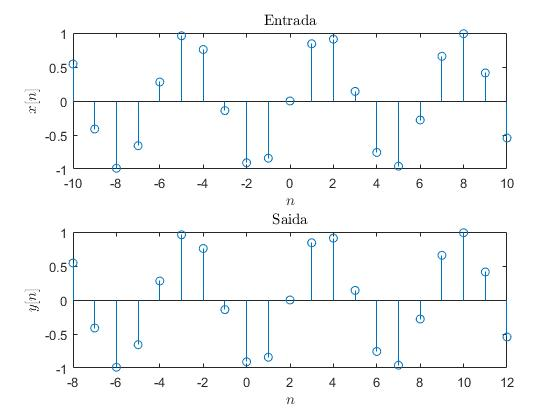
\includegraphics[scale=0.7]{img1.jpg} 
	\caption{Resposta do atrasador ideal para entrada $x[n] = sin(n)$, com $n_d = 2$.}
	\label{fig:1a}
\end{figure}

\begin{figure}[H]
	\centering
	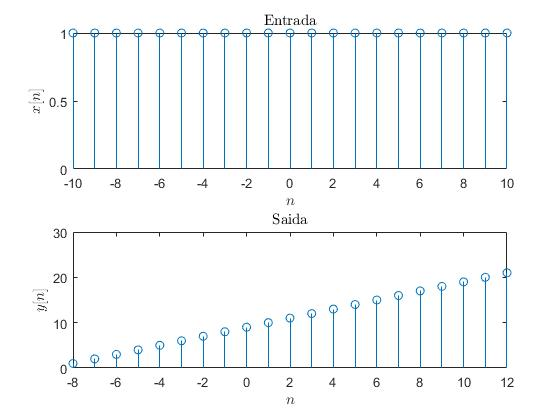
\includegraphics[scale=0.7]{img2.jpg} 
	\caption{Resposta do acumulador para entrada $x[n] = 1$.}
	\label{fig:1a}
\end{figure}

\begin{figure}[H]
	\centering
	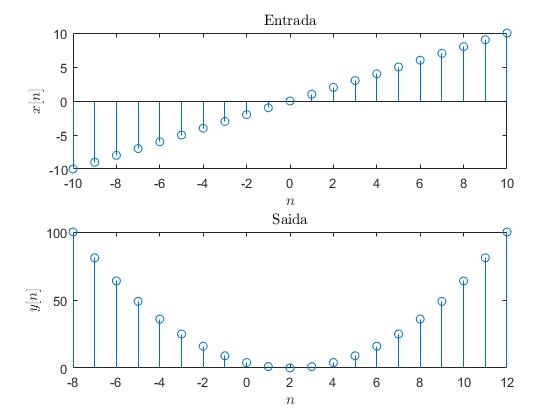
\includegraphics[scale=0.7]{img3.jpg} 
	\caption{Resposta do quadrador (exemplo de sistema não linear) para entrada $x[n] = n$.}
	\label{fig:1a}
\end{figure}

\end{document}